\section{Rotatore rigido}
Come esempio di sistema quantomeccanico molto semplice si vuole studiare in questo capitolo il \emph{rotatore rigido unidimensionale}. Un sistema di questo tipo è caratterizzato da un angolo di rotazione $\varphi$ che varia tra $0$ e $2\pi$. 
\begin{figure}[H]
    \centering
    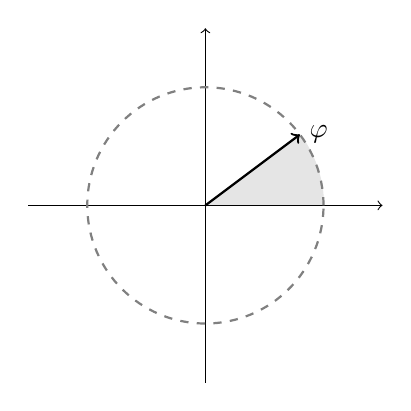
\begin{tikzpicture}[scale=1.5]
        \draw[fill=black!10,black!10] (0,0) -- (1,0) arc(0:36.8698976:1)node[anchor=west,black]{$\varphi$} (.8,.6) -- (0,0);
        \draw[->] (0,-1.5) -- (0,1.5);
        \draw[->] (-1.5,0) -- (1.5,0);
        \draw[dashed,color=gray,thick] (0,0) circle (1);
        \draw[->,thick] (0,0) -- (.8,.6);
    \end{tikzpicture}
\end{figure}
Classicamente ad un angolo di rotazione è associato un momento generalizzato $P_\varphi$. Analogamente in meccanica quantistica s vogliono definire gli operatori autoaggiunti $\hat \varphi$ e $\hat P_\varphi$. Per prima cosa, utilizzando il principio di quantizzazione, si deve imporre la relazione di commutazione imposta dalle parentesi di Poisson classiche:
\begin{equation*}
    \{\varphi,P_\varphi\}=1\qquad\Rightarrow\qquad[\hat\varphi,\hat P_\varphi]=i\hslash\hat{I}.
\end{equation*}
Si vuole che $\hat\varphi$ di origine ad una base di autoket ortonormale che si indicherà con $\ket{\varphi}$. Lo spettro di questo operatore è continuo (siccome deve rappresentare un angolo nello spazio delle configurazioni) e si suppone che valgano le seguenti relazioni (in analogia con quanto accade con $x$ nella rappresentazione di Schrödinger):
\begin{equation*}
    \bra{\varphi}\hat\varphi=\varphi\bra{\varphi},\qquad\bra{\varphi}\hat P_\varphi=-i\hslash\frac{d}{d\phi}\bra{\varphi}.
\end{equation*}
Siccome $\varphi$ rappresenta un angolo si vuole che una rotazione di $2\pi$ non modifichi lo stato del sistema ($\ket{\varphi+2\pi}=\ket{\varphi}$), questa richiesta però non è compatibile con le relazioni agli autovalori precedenti. Per questo motivo il dominio dello spettro è ristretto in $[-\pi,\pi]$. Varranno quindi le seguenti relazioni di completezza:
\begin{equation*}
    \braket{\varphi'|\varphi}=\sum_{k=\infty}^{\infty}\delta(\varphi'-\varphi+2\pi k),\qquad\int_{-\pi}^{+\pi}\ket{\varphi}d\varphi\bra{\varphi}=\hat I,
\end{equation*}
In questo modo $\varphi$ da origine ad una rappresentazione "angolare".
dove $\delta(x)$ è la delta di Dirac.
\subsection{Spettro dell'operatore momento}
Si vuole ora studiare lo spettro dell'operatore $\hat P_\varphi$. Se si suppone $\ket{p_\varphi}$ autoket di $\hat P_\varphi$ si ha:
\begin{equation*}
    \hat P_\varphi\ket{\hat P_\varphi}=\ket{\hat P_\varphi}\hat P_\varphi.
\end{equation*}
Utilizzando la rappresentazione che si è appena creata si ha:
\begin{equation*}
    \bra{\varphi}\hat P_\varphi\ket{\hat P_\varphi}=-i\hslash\frac{d}{d\phi}\braket{\varphi|P_\varphi}=\braket{\varphi|P_\varphi}P_\varphi.
\end{equation*}
Questa è di fatto un'equazione differenziale per $\braket{\varphi|P_\varphi}$ che risulta quindi:
\begin{equation*}
    \braket{\varphi|P_\varphi}=ce^{\frac{i}{\hslash}P_\varphi\varphi},
\end{equation*}
dove $c$ è una costante complessa da determinare imponendo la normalizazione degli autoket.\\
A questo punto è necessario imporre le condizioni di periodicità richiesta dalla natura angolare di $\varphi$:
\begin{equation*}
    \braket{\varphi+2\pi|P_\varphi}=\braket{\varphi|P_\varphi}\quad\Rightarrow\quad e^{\frac{i}{\hslash}2\pi P_\varphi}=1\quad\Rightarrow\quad\frac{i}{\hslash}2\pi P_\varphi=2m\pi i,\ m\in\mathbb{Z}\quad\Rightarrow\quad P_\varphi=\hslash m,\ m\in\mathbb{Z}.
\end{equation*}
\begin{proposition}
    L'operatore $\hat P_\varphi$ ha spettro discreto dato da $\{\dots,-2\hslash,-\hslash,0,\hslash,2\hslash,\dots\}$.
\end{proposition}
In questo modo la base di autoket di $\hat P_\varphi$ è rinominata:
\begin{equation*}
    \hat P_\varphi\ket{m}=\ket{m}\hslash m,\qquad\braket{\varphi|m}=\frac{e^{im\varphi}}{\sqrt{2\pi}}.
\end{equation*}
Infine si osservi che
\begin{equation*}
    \braket{\varphi|m}=\frac{e^{im\varphi}}{\sqrt{2\pi}}=e^{im\varphi}\braket{\varphi|0}=\braket{\varphi|e^{im\hat\varphi}|0}\quad\Rightarrow\quad\boxed{\ket{m}=e^{im\hat\varphi}\ket{0}}\ .
\end{equation*}
\subsection{Parità del rotatore rigido}
In generale è possibile definire l'operatore \emph{parità} e sfruttarne le proprietà per studiare un qualsivoglia sistema. Per il rotatore rigido unidimensionale la sua definizione è la seguente.
\begin{definition}
    Sia $\bra{\phi}$ un autobra di $\hat\varphi$ allora si definisce l'operatore \emph{parità} $\hat P$ tale che:
    \begin{equation*}
       \bra{\varphi}\hat P=\bra{-\varphi}.
    \end{equation*}    
\end{definition}
Da questa semplice definizione si hanno una serie di proprietà notevoli dell'operatore parità.
\begin{proposition}
    Sia $\hat P$ l'operatore parità allora valgono:
    \begin{itemize}
        \item $\hat P^2=\hat I$  o $\hat P^{-1}=\hat P$,
        \item è autoaggiunto $\hat P^*=\hat P$,
        \item il suo spettro consiste di $\pm1$.
    \end{itemize}
\end{proposition}
\begin{proof}
    La prima porprietà (nota come idempotenza) segue facilmente dal seguente conto:
    \begin{equation*}
        \bra{\varphi}\hat P\hat P=\bra{-\varphi}\hat P\bra{\varphi}=\bra{\varphi}\hat I\qquad \Rightarrow\qquad \hat P^{-1}=\hat P.
    \end{equation*}
    La proprietà $\hat P^*=\hat P$ è invece facilmente dimostrata facendo uso delle relazioni di ortonormalità:
    \begin{equation*}
        \braket{\varphi'|\hat P^*|\varphi}=\overline{\braket{\varphi|\hat P|\varphi'}}=\overline{\braket{-\varphi|\varphi'}}=\delta(\varphi+\varphi')=\braket{-\varphi'|\varphi}=\braket{\varphi'|\hat P|\varphi}.
    \end{equation*}
    Infine si può ricavare lo spettro dell'operatore parità costruendo ad'hoc i suoi autospazi. Infatti dato un qualsivoglia ket $\ket{\chi}$ e definendo
    \begin{equation}
        \boxed{\ket{\chi,\pm1}=\frac{\hat I\pm\hat P}{2}\ket{\chi}} \label{autoketParità}
    \end{equation}
     si ha che quest'ultimo ket risiede in un autospazio di $\hat P$. Infatti:
     \begin{equation*}
        \hat P\ket{\chi,\pm1}=\frac{\hat P\pm\hat P^2}{2}\ket{\chi}=\frac{\hat P\pm\hat I}{2}\ket{\chi}=(\pm1)\frac{\hat P\pm\hat P^2}{2}\ket{\chi}=\ket{\chi,\pm1}(\pm1),
     \end{equation*}
     il che, siccome $\ket{\chi}$ è arbitrario, dimostra la proposizione sul suo spettro. Per questo motivo si ha anche gli autoket della parità generano tutto lo spazio di Hilbert degli stati.
\end{proof}
Note queste proprità si può determinare come agisca questo operatore sull'operatore $\hat\varphi$ e $\hat P_\varphi$, infatti:
\begin{flalign*}
    \bra{\varphi}\hat P\hat\varphi\hat P=&\bra{-\varphi}\hat\varphi\hat P=-\varphi\bra{-\varphi}\hat P=-\varphi\bra{\varphi}\quad &\Rightarrow\quad &\boxed{\hat P\hat\varphi\hat P=-\hat\varphi}\ ,&&\\
    \bra{\varphi}\hat P\hat p_\varphi\hat P=&\bra{-\varphi}\hat p_\varphi\hat P=-i\hslash\frac{d}{d\varphi'}\bra{\varphi'=-\varphi}\hat P& & &&\\=&-i\hslash\frac{d}{d\varphi'}\bra{\varphi}=i\hslash\frac{d}{d\varphi}\bra{\varphi}=-\bra{\varphi}\hat P_\varphi \quad &\Rightarrow\quad &\boxed{\hat P\hat P_\varphi\hat P=-\hat P_\varphi}\ .&&
\end{flalign*}
Infine si può costruire, come si è fatto nella \eqref{autoketParità}, un autoket della parità a partire da quelli di $\hat P_\varphi$. Infatti $\hat P$ agendo su $\ket{m}$ risulta in:
\begin{equation*}
    \braket{\varphi|\hat P|m}=\braket{-\varphi|m}=\frac{e^{-im\varphi}}{\sqrt{2\pi}}=\braket{\varphi|-m}\quad\Rightarrow\quad\boxed{\hat{P}\ket{m}=\ket{-m}}\ ,
\end{equation*}
per cui $\ket{m}$ non appartiene a nessun'autospazio della parità a meno che $m=0$.\\
Ponendo $\eta=\pm1$ si ha che
\begin{equation}
    \boxed{
        \ket{l,\eta}=\frac{\ket{l}+\ket{-l}\eta}{\sqrt{2}}\label{lEta}
    }\ ,\qquad l\neq0,
\end{equation}
è un autoket della parità infatti:
\begin{equation*}
   \hat P \ket{l,\eta}=\frac{\hat P\ket{l}+\hat P\ket{-l}\eta}{\sqrt{2}}=\frac{\ket{-l}+\hat P\ket{l}\eta}{\sqrt{2}}\eta=\frac{\ket{-l}\eta+\hat P\ket{l}}{\sqrt{2}}=\ket{l,\eta}\eta.
\end{equation*}
L'insieme di autoket $\ket{0},\ \ket{l,\eta}$ con $l\in\mathbb{N}, \eta=\pm1$ generano quindi tutto lo spazio degli stati, inoltre formano una base ortonormale. Infatti $\ket{0}$ è chiaramente ortonormale a tutti gli altri autoket per costruzione (già i $\ket{m}$ sono tra loro ortonormali) e vale:
\begin{equation*}
    \braket{l',\eta'|l,\eta}=\frac{(\bra{l'}+\eta'\bra{-l'})(\ket{l}+\ket{-l}\eta)}{2}=\frac{\braket{l'|l}+\eta'\braket{-l'|l}+\eta\braket{l'|-l}+\eta\eta'\braket{-l'|-l}}{2},
\end{equation*}
siccome $l$ è maggiore di $0$ si ha che i termini $\braket{l'|-l}$ e $\braket{-l'|l}$ sono sempre nulli. In questo modo:
\begin{equation*}
    \braket{l',\eta'|l,\eta}=\frac{1+\eta\eta'}{2}\delta_{l,l'}=\delta_{l,l'}\delta_{\eta,\eta'}
\end{equation*}
il che dimostra le relazioni di ortonormalità.\\
Questa trattazione permette di ottenere due semplici formule utili per molti problemi fisici.
\begin{proposition}
    Valgono le seguenti relazioni:
    \begin{equation*}
        \ket{l,+1}=\sqrt{2}\cos(l\hat \varphi)\ket{0},\qquad\ket{l,-1}=i\sqrt{2}\sin(l\hat \varphi)\ket{0}.
    \end{equation*}
\end{proposition}
\begin{proof}
    Dalle definizioni \eqref{lEta} di $\ket{l,\pm1}$ si ha:
    \begin{flalign*}
        \ket{l,+1}&=\ket{l,+1}=\frac{\ket{l}+\ket{-l}}{\sqrt{2}}=\frac{e^{il\hat\varphi}+e^{-il\hat\varphi}}{\sqrt{2}}\ket{0}=\sqrt{2}\cos(l\hat \varphi)\ket{0}\\
        \ket{l,-1}&=\ket{l,-1}=\frac{\ket{l}-\ket{-l}}{\sqrt{2}}=\frac{e^{il\hat\varphi}-e^{-il\hat\varphi}}{\sqrt{2}}\ket{0}=i\sqrt{2}\sin(l\hat \varphi)\ket{0}
    \end{flalign*}
\end{proof}
Questo risultato consente di ottenere anche la rappresentazione dei nuovi autoket:
\begin{equation*}
    \boxed{\braket{\varphi|l,+1}=\frac{\cos(l\varphi)}{\sqrt{\pi}}}\ ,\qquad\boxed{\braket{\varphi|l,-1}=\frac{i\sin(l\varphi)}{\sqrt{\pi}}}\ ,
\end{equation*}
in questo modo si conclude quanto di può dire sulla cinematica del rotatore rigido.
\begin{example}
    Un rotatore rigido può essere utilizzato per modellizzare un dipolo elettrico di carica $q$ e la cui separazione tra le cariche è $l$. Questo se viene inserito in un campo elettrico esterno $\underline E$ avrà un'energia di accoppiamento con il campo elettrico:
    \begin{equation*}
        W=|\underline{E}| ql \cos(\varphi).
    \end{equation*}
    In meccanica quantistica questa interazione è descritta dall'operatore 
    \begin{equation*}
        \hat W=|\underline{E}| ql \cos(\hat\varphi).
    \end{equation*}
    I calcoli che si debbono fare con questo operatore sono semplificati da quanto appena descritto.
\end{example}
\subsection{Hamiltoniano del rotatore rigido libero}
Classicamente si ha che un rotatore rigido libero ha un'hamiltoniana data da:
\begin{equation*}
    H=\frac{P^2_\varphi}{2I},
\end{equation*}
dove $P_\varphi$ è il momento generalizzato associato all'angolo $\varphi$ e $I$ è il momento d'inerzia del rotatore. In meccanica quantistica questo si traduce in un operatore hamiltoniano:
\begin{equation*}
    \hat H=\frac{\hat P^2_\varphi}{2I}.
\end{equation*}
Siccome $\hat H$ è una funzione di $\hat P_\varphi$ allora gli autoket di quest'ultimo lo sono anche per l'operatore hamiltoniano, si ha quindi:
\begin{equation*}
    \hat H\ket{m}=\frac{\hat P^2_\varphi\ket{m}}{2I}=\ket{m}\frac{\hslash^2m^2}{2I}.
\end{equation*}
Lo spettro energetico è quindi dato da $E_n=\frac{\hslash^2n^2}{2I}$ con $n\geq0$ intero ed è doppiamente degenere poichè ogni autospazio di autovalore $E_n$ si è di dimensione $2$ generato dagli autoket $\ket{\pm n}$.\\Inoltre l'operatore hamiltoniano, dipendendo quadraticamente da $\hat P_\varphi$, è invariante per parità, ossia:
\begin{equation*}
    \hat P\hat H \hat P=\frac{(\hat P\hat P_\varphi\hat P)^2}{2I}=\frac{(-\hat P_\varphi)^2}{2I}=\hat H.
\end{equation*}
Infine va osservato che, siccome vale $\hat P^{-1}=\hat P$, allora l'invarianza per parità è equivalente alla commutatività dei due operatori:
\begin{equation*}
    \hat P[\hat H,\hat P]=\hat P\hat H\hat P-\hat P\hat P\hat H=\hat H-\hat H=0\quad \Rightarrow \quad [\hat H,\hat P]=0.
\end{equation*}
In questo modo si è determinato che $\hat H$ e $\hat P$ formano un insieme completo di operatori autoaggiunti e commutanti e per questo è ammessa un'unica base simultanea di autoket di entrambi. Questa è proprio la base $\ket{0},\ \ket{l,\eta}$ con $l\in\mathbb{N}, \eta=\pm1$, infatti:
\begin{equation*}
    \hat H\ket{l,\eta}=\frac{\hat H\ket{l}+\hat H\ket{-l}\eta}{\sqrt{2}}=\frac{\ket{l}E_l+\ket{-l}\eta E_l}{\sqrt{2}}=\ket{l,\eta}E_l.
\end{equation*}
